\documentclass{article}

\usepackage[utf8]{inputenc}

\usepackage[backend=biber,style=authoryear,]{biblatex}
%%%%%%%%%%%%%%%%%%%%%%%%%%%%%%%%%%%%%%%%%
% Arsclassica Article
% Structure Specification File
%
% This file has been downloaded from:
% http://www.LaTeXTemplates.com
%
% Original author:
% Lorenzo Pantieri (http://www.lorenzopantieri.net) with extensive modifications by:
% Vel (vel@latextemplates.com)
%
% License:
% CC BY-NC-SA 3.0 (http://creativecommons.org/licenses/by-nc-sa/3.0/)
%
%%%%%%%%%%%%%%%%%%%%%%%%%%%%%%%%%%%%%%%%%

%----------------------------------------------------------------------------------------
%	REQUIRED PACKAGES
%----------------------------------------------------------------------------------------

\usepackage[
nochapters, % Turn off chapters since this is an article        
beramono, % Use the Bera Mono font for monospaced text (\texttt)
eulermath,% Use the Euler font for mathematics
pdfspacing, % Makes use of pdftex’ letter spacing capabilities via the microtype package
dottedtoc % Dotted lines leading to the page numbers in the table of contents
]{classicthesis} % The layout is based on the Classic Thesis style

\usepackage{arsclassica} % Modifies the Classic Thesis package

\usepackage[T1]{fontenc} % Use 8-bit encoding that has 256 glyphs

\usepackage[utf8]{inputenc} % Required for including letters with accents

\usepackage{graphicx} % Required for including images
\graphicspath{{Figures/}} % Set the default folder for images

\usepackage{enumitem} % Required for manipulating the whitespace between and within lists

\usepackage{lipsum} % Used for inserting dummy 'Lorem ipsum' text into the template

\usepackage{subfig} % Required for creating figures with multiple parts (subfigures)

\usepackage{amsmath,amssymb,amsthm} % For including math equations, theorems, symbols, etc

\usepackage{multirow} % for including eqs in multirows

\usepackage{varioref} % More descriptive referencing

\usepackage{floatflt,epsfig} % for including figure in the text

\usepackage{wrapfig}
%----------------------------------------------------------------------------------------
%	THEOREM STYLES
%---------------------------------------------------------------------------------------

\theoremstyle{definition} % Define theorem styles here based on the definition style (used for definitions and examples)
\newtheorem{definition}{Definition}

\theoremstyle{plain} % Define theorem styles here based on the plain style (used for theorems, lemmas, propositions)
\newtheorem{theorem}{Theorem}

\theoremstyle{remark} % Define theorem styles here based on the remark style (used for remarks and notes)

%----------------------------------------------------------------------------------------
%	HYPERLINKS
%---------------------------------------------------------------------------------------

\hypersetup{
%draft, % Uncomment to remove all links (useful for printing in black and white)
colorlinks=true, breaklinks=true, bookmarks=true,bookmarksnumbered,
urlcolor=webbrown, linkcolor=RoyalBlue, citecolor=webgreen, % Link colors
pdftitle={}, % PDF title
pdfauthor={\textcopyright}, % PDF Author
pdfsubject={}, % PDF Subject
pdfkeywords={}, % PDF Keywords
pdfcreator={pdfLaTeX}, % PDF Creator
pdfproducer={LaTeX with hyperref and ClassicThesis} % PDF producer
}
 
\addbibresource{sample.bib}

%\bibliography{sample}
\title{Report for Bioscience Faculty\\Ruperto Carola University of Heidelberg}
\author{Carla Filosa}
\date{January 2018}

\begin{document}

\maketitle
\setcounter{tocdepth}{2} % Set the depth of the table of contents to show sections and subsections only

\tableofcontents % Print the table of contents

%\listoffigures % Print the list of figures

%\listoftables % Print the list of tables
\section{Introduction}
\section{What is a cell assembly?}
The fundamental concept of cell assembly was introduced by Hebb in the 1949. After more than six decades this idea continue to play a key role in our understanding of how neural physiology may link to cognitive function.
In few words a cell assembly refers to a group of neurons which, by functionally organizing into a temporally coherent set, come to represent mental or perceptual entities, thereby forming the basis  of neural coding and computation (\cite{Hebb}). However this definition is not precise and under the term cell assembly scientists have for long years included anything from precise zero-phase-lag spike synchronization in a defined subset of neurons to temporally coherent changes in average firing rates or larger time scale. That means that for different time scales, different type of assemblies exist associated to the different neurons patterns.
In 2017 Russo and Durstewitz introduced a method able to detect different typologies of assemblies in multi-cell electrophysiological recording being able to distinguish different processes at different time scales, and as well to remove many non-stationary artefacts that plague data analysis in neuroscience.
The detected pattern occur with a frequency that is higher the chance level and can be generated either by anatomically or functionally connected groups of neurons.

In figure (\ref{fig: AsEx}) we see an example of different possible detectable patterns . 
\begin{figure}[!ht]
  \begin{center}
    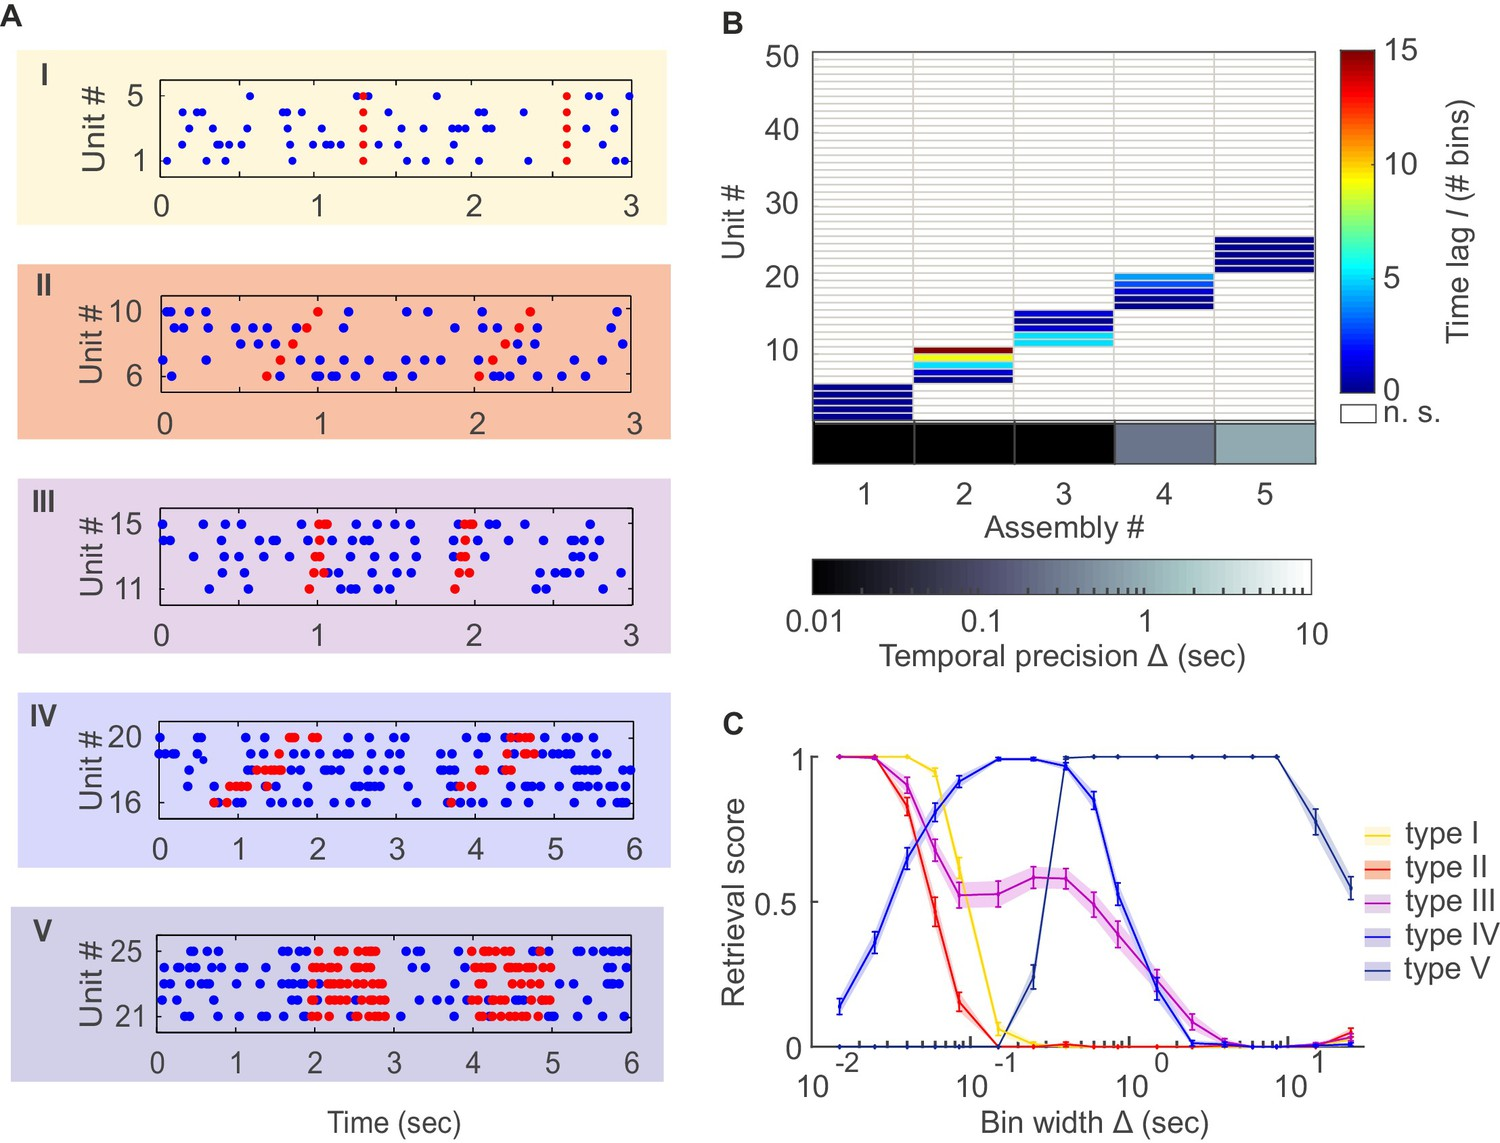
\includegraphics[width=1\textwidth]{AsEx1}
  \end{center}
\caption{\footnotesize{Detection of assemblies defined by different degrees of temporal precision, scale, and internal structure. Different assembly types in simulated non-stationary spike train: I - highly precise lag-0 synchronization; II- precise sequential pattern; III - precise-spike-time patterns without clear sequential structure; IV - rate pattern with temporal structure; V - simultaneous rate increase. Figure reproduced and modified from (\cite{RussoDurstewitz})}}
\label{fig: AsEx}
\end{figure}


\section{The ensemble detection method}
We won't go in the details of the method, that are explained in (\cite{RussoDurstewitz}), we rather show a schematic idea trough simple but fundamental steps. We show the novelty and the strength of the method instead, applying it on really data, and exploring the different possible applications as well investigating the kind of information that the assemblies carry on.
The method is based on counting spike occurrences of two units A,B. The idea proposed is using  multiple bin widths $\Delta$ and time lags $l$ to capture different neural patterns at different time scales. Find patterns means find objects that are not independent each other, given that they are generated by anatomically of functionally connected groups of neurons. Keeping in mind this definition, the core of algorithm is easy to understand if we have only one basic mathematical notion:
\begin{itemize}
    \item For two independent data set $A, B$ the joint distribution of spike occurrences $p(A,B)$ at specific lag $l$ can be factor int single unit marginal distribution $p(A,B)=p(A)p(B)$
\end{itemize}
For spiking data we have a time series $\{c_t\}$ of spike counts of length $T$, we should chose a bin width $\Delta$ small enough to guarantee: $c_t \in \{0,1\}$, $\#_A$ and $\#_B$ is the total number of spikes of $A$ and $B$ respectively. So the null Hypothesis ($H_0$) of independence asserts the following:
\begin{itemize}
    \item The joint spike count $\#_{A,B}$ at the time lag $l$ follows a hypergeometric distribution with mean: $\mu_{A,B} = \frac{\#_A \#_B}{T-l}$ and variance $\sigma^2_{AB,l}$
\end{itemize}
The algorithm is provided of a remedy for the non-stationarity based on the assumptionthat the non-stationarity affect the data omogeneously, namely without a preferred lag direction. Under this condition one can remove the non-stationarity using the difference statistic, namely:
$$\#_{ABBA,l}=\#_{AB,l}-\#_{AB,-l}$$

\section{Results and possible applications}
\subsection{What the assemblies confirm?}
\subsection{Directionality}
\section{Conclusion}
\newpage

\printbibliography
%\renewcommand{\refname}{\spacedlowsmallcaps{Brief list of principle references}} % For modifying the bibliography heading

%\bibliographystyle{unsrt}


%\bibliography{sample.bib} % The file containing the bibliography
%\begin{thebibliography}{triangle}

%\bibitem[Russo, Durstewitz, 2017]{RussoDurstewitz}
%E. Russo, D. Durstewitz: 
%\newblock{Cell assemblies at multiple time scales }
%\newblock{\textit{2nd ed. Chapman \& Hall,London}. (1989) }



%\end{thebibliography}


\end{document}



